\documentclass{standalone}
\usepackage{tikz}
\usetikzlibrary{patterns, positioning}


\begin{document}
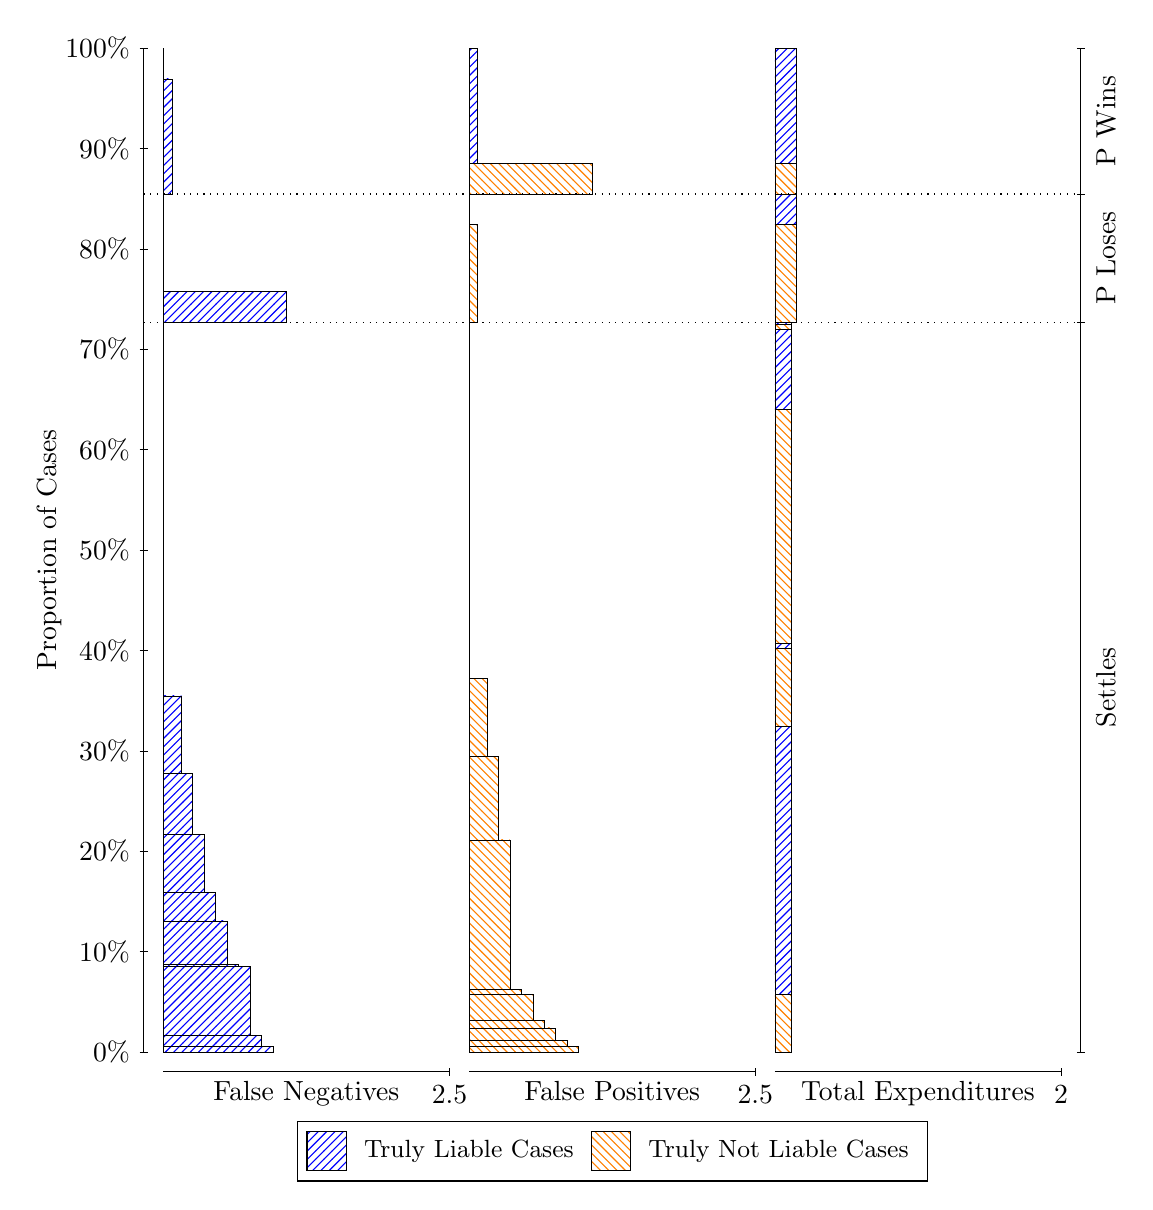
\begin{tikzpicture}
\draw[black, very thin] (1.5,1.75) -- (1.5,14.5);
\node[rotate=90, text=black, anchor=center] at (0.3, 8.125) {Proportion of Cases};
\draw[black, very thin] (1.45,1.75) -- (1.55,1.75);
\node[text=black, anchor=east] at (1.45, 1.75) {0\%};
\draw[black, very thin] (1.45,3.025) -- (1.55,3.025);
\node[text=black, anchor=east] at (1.45, 3.025) {10\%};
\draw[black, very thin] (1.45,4.3) -- (1.55,4.3);
\node[text=black, anchor=east] at (1.45, 4.3) {20\%};
\draw[black, very thin] (1.45,5.575) -- (1.55,5.575);
\node[text=black, anchor=east] at (1.45, 5.575) {30\%};
\draw[black, very thin] (1.45,6.85) -- (1.55,6.85);
\node[text=black, anchor=east] at (1.45, 6.85) {40\%};
\draw[black, very thin] (1.45,8.125) -- (1.55,8.125);
\node[text=black, anchor=east] at (1.45, 8.125) {50\%};
\draw[black, very thin] (1.45,9.4) -- (1.55,9.4);
\node[text=black, anchor=east] at (1.45, 9.4) {60\%};
\draw[black, very thin] (1.45,10.675) -- (1.55,10.675);
\node[text=black, anchor=east] at (1.45, 10.675) {70\%};
\draw[black, very thin] (1.45,11.95) -- (1.55,11.95);
\node[text=black, anchor=east] at (1.45, 11.95) {80\%};
\draw[black, very thin] (1.45,13.225) -- (1.55,13.225);
\node[text=black, anchor=east] at (1.45, 13.225) {90\%};
\draw[black, very thin] (1.45,14.5) -- (1.55,14.5);
\node[text=black, anchor=east] at (1.45, 14.5) {100\%};

\draw[black, very thin] (13.4,1.75) -- (13.4,14.5);
\draw[black, very thin] (13.35,1.75) -- (13.45,1.75);
\node[anchor=west] at (13.35, 1.75) {};
\draw[black, very thin] (13.35,11.016) -- (13.45,11.016);
\node[anchor=west] at (13.35, 11.016) {};
\draw[black, very thin] (13.35,12.646) -- (13.45,12.646);
\node[anchor=west] at (13.35, 12.646) {};
\draw[black, very thin] (13.35,14.5) -- (13.45,14.5);
\node[anchor=west] at (13.35, 14.5) {};

\draw[black, very thin, pattern color=blue, pattern=north east lines] (1.75,1.75) rectangle (3.1398,1.817);
\draw[black, very thin, pattern color=blue, pattern=north east lines] (1.75,1.817) rectangle (2.9944,1.9619);
\draw[black, very thin, pattern color=blue, pattern=north east lines] (1.75,1.9619) rectangle (2.8491,2.8322);
\draw[black, very thin, pattern color=blue, pattern=north east lines] (1.75,2.8322) rectangle (2.7037,2.8613);
\draw[black, very thin, pattern color=blue, pattern=north east lines] (1.75,2.8613) rectangle (2.5584,3.4144);
\draw[black, very thin, pattern color=blue, pattern=north east lines] (1.75,3.4144) rectangle (2.4131,3.7743);
\draw[black, very thin, pattern color=blue, pattern=north east lines] (1.75,3.7743) rectangle (2.2678,4.5175);
\draw[black, very thin, pattern color=blue, pattern=north east lines] (1.75,4.5175) rectangle (2.1224,5.2837);
\draw[black, very thin, pattern color=blue, pattern=north east lines] (1.75,5.2837) rectangle (1.9771,6.2717);
\draw[black, very thin, pattern color=orange, pattern=north west lines] (1.75,6.2717) rectangle (1.75,11.016);
\draw[black, very thin, pattern color=blue, pattern=north east lines] (1.75,11.016) rectangle (3.3123,11.407);
\draw[black, very thin, pattern color=orange, pattern=north west lines] (1.75,11.407) rectangle (1.75,12.646);
\draw[black, very thin, pattern color=blue, pattern=north east lines] (1.75,12.646) rectangle (1.859,14.109);
\draw[black, very thin, pattern color=orange, pattern=north west lines] (1.75,14.109) rectangle (1.75,14.5);
\draw[black, very thin, pattern color=orange, pattern=north west lines] (5.6333,1.75) rectangle (7.0231,1.817);
\draw[black, very thin, pattern color=orange, pattern=north west lines] (5.6333,1.817) rectangle (6.8777,1.8999);
\draw[black, very thin, pattern color=orange, pattern=north west lines] (5.6333,1.8999) rectangle (6.7324,2.0559);
\draw[black, very thin, pattern color=orange, pattern=north west lines] (5.6333,2.0559) rectangle (6.5871,2.147);
\draw[black, very thin, pattern color=orange, pattern=north west lines] (5.6333,2.147) rectangle (6.4417,2.4773);
\draw[black, very thin, pattern color=orange, pattern=north west lines] (5.6333,2.4773) rectangle (6.2964,2.5416);
\draw[black, very thin, pattern color=orange, pattern=north west lines] (5.6333,2.5416) rectangle (6.1511,4.4447);
\draw[black, very thin, pattern color=orange, pattern=north west lines] (5.6333,4.4447) rectangle (6.0057,5.5065);
\draw[black, very thin, pattern color=orange, pattern=north west lines] (5.6333,5.5065) rectangle (5.8604,6.4946);
\draw[black, very thin, pattern color=blue, pattern=north east lines] (5.6333,6.4946) rectangle (5.6333,11.016);
\draw[black, very thin, pattern color=orange, pattern=north west lines] (5.6333,11.016) rectangle (5.7423,12.256);
\draw[black, very thin, pattern color=blue, pattern=north east lines] (5.6333,12.256) rectangle (5.6333,12.646);
\draw[black, very thin, pattern color=orange, pattern=north west lines] (5.6333,12.646) rectangle (7.1957,13.037);
\draw[black, very thin, pattern color=blue, pattern=north east lines] (5.6333,13.037) rectangle (5.7423,14.5);
\draw[black, very thin, pattern color=orange, pattern=north west lines] (9.5167,1.75) rectangle (9.721,2.4773);
\draw[black, very thin, pattern color=blue, pattern=north east lines] (9.5167,2.4773) rectangle (9.721,5.8877);
\draw[black, very thin, pattern color=orange, pattern=north west lines] (9.5167,5.8877) rectangle (9.721,6.8758);
\draw[black, very thin, pattern color=blue, pattern=north east lines] (9.5167,6.8758) rectangle (9.721,6.9428);
\draw[black, very thin, pattern color=orange, pattern=north west lines] (9.5167,6.9428) rectangle (9.721,9.9078);
\draw[black, very thin, pattern color=blue, pattern=north east lines] (9.5167,9.9078) rectangle (9.721,10.923);
\draw[black, very thin, pattern color=orange, pattern=north west lines] (9.5167,10.923) rectangle (9.721,10.987);
\draw[black, very thin, pattern color=blue, pattern=north east lines] (9.5167,10.987) rectangle (9.721,11.016);
\draw[black, very thin, pattern color=orange, pattern=north west lines] (9.5167,11.016) rectangle (9.7892,12.256);
\draw[black, very thin, pattern color=blue, pattern=north east lines] (9.5167,12.256) rectangle (9.7892,12.646);
\draw[black, very thin, pattern color=orange, pattern=north west lines] (9.5167,12.646) rectangle (9.7892,13.037);
\draw[black, very thin, pattern color=blue, pattern=north east lines] (9.5167,13.037) rectangle (9.7892,14.5);
\draw[black, dotted] (1.5,11.016) -- (13.4,11.016);
\draw[black, dotted] (1.5,12.646) -- (13.4,12.646);
\draw[black, very thin] (1.75,1.5) -- (5.3833,1.5);
\node[text=black, anchor=north] at (3.5667, 1.5) {False Negatives};
\draw[black, very thin] (5.3833,1.45) -- (5.3833,1.55);
\node[text=black, anchor=north] at (5.3833, 1.45) {2.5};

\draw[black, very thin] (5.6333,1.5) -- (9.2667,1.5);
\node[text=black, anchor=north] at (7.45, 1.5) {False Positives};
\draw[black, very thin] (9.2667,1.45) -- (9.2667,1.55);
\node[text=black, anchor=north] at (9.2667, 1.45) {2.5};

\draw[black, very thin] (9.5167,1.5) -- (13.15,1.5);
\node[text=black, anchor=north] at (11.333, 1.5) {Total Expenditures};
\draw[black, very thin] (13.15,1.45) -- (13.15,1.55);
\node[text=black, anchor=north] at (13.15, 1.45) {2};

\node[text=black, centered, rotate=90] at (13.72, 6.3832) {Settles};
\node[text=black, centered, rotate=90] at (13.72, 11.831) {P Loses};
\node[text=black, centered, rotate=90] at (13.72, 13.573) {P Wins};

\draw (7.449999999999999,1.5) node[draw=none] (baseCoordinate) {};
\begin{scope}[align=center]
        \matrix[scale=0.5, draw=black, below=0.5cm of baseCoordinate, nodes={draw}, column sep=0.1cm]{
            \node[rectangle, draw, minimum width=0.5cm, minimum height=0.5cm, pattern color=blue, pattern=north east lines] {}; &
            \node[draw=none, font=\small, text=black] (B) {Truly Liable Cases}; &
            \node[rectangle, draw, minimum width=0.5cm, minimum height=0.5cm, pattern color=orange, pattern=north west lines] {}; &
            \node[draw=none, font=\small, text=black] (B) {Truly Not Liable Cases}; \\
            };
\end{scope}

\end{tikzpicture}
\end{document}